\documentclass[12pt]{article}

\usepackage[T1]{fontenc} 
\usepackage[utf8]{inputenc}
\usepackage[francais]{babel}
\usepackage{graphicx}
\usepackage{hyperref}
\usepackage{url}
\usepackage{color}
\usepackage[usenames,dvipsnames]{xcolor}
\usepackage{alltt}
\usepackage{tocbibind}


\title{Rapport Final projet EDD}
\author{Pinero, Borde, Bonnet}

\begin{document}
\maketitle
\tableofcontents

\newpage

\section{Le projet}
\subsection{Pr\'esentation}
Le projet ce compose de plusieurs parties de d\'eveloppement sur un sujet
commun, le jeu du 2048. Ce jeu conciste \`a additionner des tuiles de m\^eme
puissance de 2, sur un plateau de 16 tuiles, jusqu'\`a ce que le plateau soit
plein et qu'aucune addition ne soit possible. Le but du jeu et d’arriver \'a
construire une brique de valeur la plus grande possible (2048, 4096,
8192, \ldots)
\par 
\emph{\color{red}POURQUOI PAS AJOUTER UNE PHOTO EXEMPLE ?!}
\subsection{Le sujet}
Dans le projet nous avons eu \`a r\'ealiser dans un premier temps l'ensemble du
moteur du jeu et quelques tests qui nous garantisent au maximum la soliditer de notre code 
pendant le d\'eveloppement. Dans un deuxi\`eme temps, nous devions faire la
\og critique \fg{} du developpement de la premi\`ere partie faite par
d'autres groupes bas\'e sur une grille d'evaluation qui nous a \'et\'e
fourni. Ensuite nous avons r\'ealiser un ensemble de strat\'egie de jeu qui
sont capable de jouer de mani\`ere autonome une partie enti\`ere. Ces strat\'egies doivent \`a chaque tours calculer le meilleur
prochain coups pour atteindre le plus grand score possible. La derni\`ere partie
du projet conciste \`a r\'ealis\'e une v\'eritable interface graphique pour
jouer au jeu.

\newpage
\section{D\'eveloppement du 2048 et tests}
Pour le d\'eveloppement du 2048, le langage de programmation \'etait impos\'e,
nous devions utilis\'e le langage C. Chaque groupe à d\^u fournir les sources
permettant de g\'en\'erer une biblioth\`eque libgrid.a (impl\'ementant les
fonctions d'\'ecrites dans grid.h en annexe \ref{grid_h}) ainsi qu’un
ex\'ecutable permettant de jouer au 2048 dans la console. En plus de ça, nous
avons r\'ealis\'e des tests pour v\'erifier toutes les fonctions
impl\'ement\'es.\par

Avant de commencer le travail de d\'eveloppement, nous avons utilis\'e un
outil de gestion de versions d\'ecentralis\'e pour que chaque membre du groupe
puisse avoir acc\'es \`a chaque instant \`a la derni\`ere version du projet.
Pour ça nous avons choisit le logiciel \href{http://git-scm.com/}{GIT}, et la plateforme
\href{http://github.com/}{GitHub}. Les sources du projet ont \'et\'e disponible tout
au long du d\'eveloppement \href{http://github.com/kamneo/EDD_project}{ici}.\par

En ce qui concerne l'arborescence de notre projet, nous avons d\'ecid\'e d'avoir
une organisation bien pr\'ecise pour quelle puisse \^etre le plus possible
g\'en\'erique, c'est \'a dire quelle s'adapte aux \'evolutions du projet.
Mais surtout pour quelle soit le plus clair possible.

\begin{alltt}
{\color{gray}
EDD_projet/        # Racine du projet
    bin/           # Fichiers ex\'ecutables.
    build/         # Fichiers de compilation du projet
    include/       # Fichiers .h des librairies g\'en\'er\'es
    lib/           # Librairies
    src/           # Fichiers tous les fichiers sources
        2048/      # Fichiers sources de l'interface graphique
        grid/      # Fichiers du moteur de jeu
            tests/ # Fichiers qui testent le moteur de jeu
}
\end{alltt}

\par

Tout au long du d\'eveloppement du projet, tous les membres du groupe se sont
mis d'accord sur le fait d'utiliser l'outils \href{http://www.cmake.org/}{CMake}
pour compiler le projet, g\'en\'erer les Makefiles qui servent eux-m\^emes \`a g\'en\'erer les
ex\'ecutables, les librairies et ex\'ecuter les tests.

\subsection{Le developpement de grid.c}
En ce qui concerne le d\'eveloppement de grid.c, qui est le moteur du jeu,
c'\'et\'e relativement simple. Les fonctions qui ont m\'erit\'e une r\'eflexion
s\'erieuse sont \og do\_move() \fg{} et \og can\_move() \fg{}. Pour ces
fonctions nous devions limit\'e au mieux la duplication de code et la compl\'exit\'e de
l'algorithme. Chose que nous n'avions au final pas tr\`es bien reussi, mais nous
veront dans la partie \ref{notre_etude}.

\subsubsection{Implementation de \og can\_move \fg{}}
Pour cette fonction, nous avons choisi l'algorithme suivant :

\begin{alltt}
{\color{gray}
Si la direction donn\'ee est \og UP \fg{} ou \og DOWN \fg{} alors
    Pour chaque colonne faire :
        Pour chaque tuile de la colonne faire :
            Si la tuille pr\'ec\'edente est \'egale \`a la courante
                retourner vrai
 		
            Si la tuille courante et non vide 
                   et qu'il y a une tuille vide dans la colonne
                retourner vrai	    	
Si la direction donn\'ee est \og RIGHT \fg{} ou \og LEFT \fg{} alors
    Pour chaque ligne faire 
        Pour chaque tuile de la ligne faire
            Si la tuille pr\'ec\'edente est \'egale \`a la courante
                retourner vrai
 		
            Si la tuille courante et non vide alors
                   et qu'il y a une tuille vide dans la ligne
                retourner vrai	    	
retourner faux
}
\end{alltt}

C'est la que l'on peut voir que nous avons commit une erreur nous n'aurions
pas du partir sur un algo qui traite séparement les direction haut/bas et droite/gauche.

Cette fonction est utilis\'ee \'a plusieurs reprises dans d'autres fonction
comme par exemple \og game\_over \fg{} ou \og do\_move \fg{}. d'o\`u
l'importance qu'elle n'ai pas une trop grande comp\`exit\'e de calcul.

\subsubsection{Implementation de \og do\_move \fg{}}
Pour cette fonction, nous avons choisi l'algorithme suivant :
\begin{alltt}
{\color{gray}
Si la direction donn\'ee ne peut pas \^etre jouer
    Ne rien faire
    
    
Si la direction donn\'e est \og UP \fg{} ou \og DOWN \fg{} alors
    Pour chaque colonne faire :
        Pour chaque tuile de la colonne faire :
            Si la tuille pr\'ec\'edente est \'egale \`a la courante
                On fusionne les deux tuilles
                On modifie le score de la partie
            
            Si la tuille courante est vide alors
            	On change sa place avec la premi\`ere tuille non vide
            	
Si la direction donn\'ee est \og RIGHT \fg{} ou \og LEFT \fg{} alors
    Pour chaque ligne faire 
        Pour chaque tuile de la ligne faire :
            Si la tuille pr\'ec\'edente est \'egale \`a la courante
                On fusionne les deux tuilles
                On modifie le score de la partie
            
            Si la tuille courante est vide alors
            	On change sa place avec la premi\`ere tuille non vide
}
\end{alltt}

\subsection{L'afficage de la grille dans la console}
Pour l'affichage de la grille dans la console, nous avons eu plusieurs version
et design. La toute premi\`ere version \'etait une simple grille dans la console
o\`u \'etait affich\'e le score et les valeurs des tuilles. Dans cette version
nous devions jouer avec les lettres Z, Q, S et D du clavier car dans le language C, la
fonction \og scanf \fg{} de la librairie \og stdio \fg{} qui permet de
lire l'entr\'ee standard, ne prend pas en compte les fl\`eches du clavier.
En annexe vous touverai une capture d'ecran de cette version.\par
Dans une deuxim\`eme version, nous avions d\'ecid\'e de mettre des couleurs dans
les tuilles en fonction de leurs valeurs. (\`a voir en annexe \ref{grille_couleur}).\par
Enfin pour r\'epondre correctement au sujet, nous avons utilis\'e la librairie
\og NCurses \fg{}. L'utilisation de cette librairie nous a permis de se
lib\'erer de deux de nos difficult\'es. La premi\`ere \'etait celle que nous devions jouer
avec des lettres et non les fl\`eches du clavier, la seconde \'etait que nous
n'avions d'affichage dynamique de la grille \`a chaque coup. Pour \^etre plus
clair, lorsqu'on jou\'e un coups avec les deux premi\`eres version de
l'affichage, la grille du coup pr\'ecedent \'etait toujours pr\'esent dans la
console. D\'esormais, la console n'affiche plus qu'une grille et elle met \`a
jour apr\`es chaque coups.\par

La version ncurses de notre projet n'a cependant pas été trés facile à implementer.
Ce genre de librairie demande un grand nombre d'initialisation de variable qui rende
difficile la conservation d'un code propre mais aussi qui multiplie les risques de fuite memoire.

\subsection{Les tests}
Les Tests sont \'ecrit pour confronter une r\'ealisation \`a sa sp\'ecification.
Le test d\'efinit un crit\`ere d’arr\^et (\'etat ou sorties \`a l’issue de
l’ex\'ecution) et permet de statuer sur le succ\`es ou sur l’\'echec d’une
v\'erification. Gr\^ace \`a la sp\'ecification, on est en mesure de faire
correspondre un \'etat d’entr\'ee donn\'e \`a un r\'esultat ou \`a une sortie.
Le test permet de v\'erifier que la relation d’entr\'ee / sortie donn\'ee par la
sp\'ecification est bel et bien r\'ealis\'ee.
\cite{Test_unitaire}

\par Sur ce principe nous avons r\'ealis\'e un test par fonction d\'ecrite dans
le fichier \og grid.h \fg{} et un test sur la r\'ealisation de plusieurs parties
qui s'ex\'ecutent avec une strat\'egie basique qui consiste \`a jouer a gauche
si on le peut sinon \`a droite, sinon en haut enfin en bas. Ainsi lorsqu'on fait
des modifications de l'une de ces fonctions, nous nous assurons que cela n'a en
rien chang\'e \`a la v\'eracit\'e des r\'esultats. L'ex\'ecution des tests
s'\'effectue avec la commande \og make test \fg{}. L'utilisation de l'outil \og CMake \fg{} nous permet d'avoir un affichage complet \`a la fin
des tests sur leurs r\'esultats pour savoir s'ils sont pass\'es avec succ\`es
ou non (exemple en annexe \ref{test}).

\par Comme dis pr\'ec\'edement, chaque test est sp\'ecifique \`a une fonction.
\begin{itemize}
  \item La cr\'eation d'une grille et sont initialisation correcte.
  \item L'homog\'en\'eit\'e de la fonction add\_tile, c'est \`a dire que la
  probabilit\'e que la tuile g\'en\'er\'e soit bien de $
  \frac{1}{le\ nombre\ de\ tuille} $ avec un marge de 0.05\%.
  \item La v\'eracit\'e des fonctions \og game\_over \fg{} et \og can\_move
  \fg{}
  \item La bonne ex\'ecution des mouvements dans chaque direction.
  \item Enfin l'ex\'ecution sans erreur de 1000 parties.
\end{itemize}

\newpage
\section{Relectures critiques}
\`A l’issue de la premi\`ere phase de travail, chaque groupe ont d\^u relire le
code produit par trois autres groupes. Pour chaque groupe \`a relire, on a
rempli un formulaire d’\'ealuation. Ce formulaire d’\'ealuation nous a \'et\'e
fourni par notre charg\'e de TD.

\par Cette feuille d'\'evaluation \'etait compos\'ee de 13 questions orient\'ees
sur trois axes. Le point de vue utilisateur, qui pousse \`a v\'erifier
principalement la propet\'e de l'archive, que la compilation ne g\'en\`ere pas
d'erreur et qu'il y a un fichier \og README \fg{} pour expliquer l'utilisation
du programme si ce n'est pas \'evident. Dans un deuxi\`eme temps, d'un point de
vu fonctionnel, nous devions v\'erifier si le programme ne pr\'esente pas de
bogue ou de fuite m\'emoire. Enfin, d'un point de vue programmation, nous
devions porter notre attention sur les patrons de conception (ou \textit{design
patterns} en anglais).

\subsection{Les relectures que nous avons r\'ealis\'e}
Nous avons eu \`a faire la relecture des groupes A, D et G. Comme nous sommes
trois, nous nous sommes divis\'e le travail et avons \'evalu\'e un groupe
chacun. Nous nous sommes ensuite concert\'e pour harmoniser nos commentaires.
Cette relecture f\^ut tr\`es int\'eressente car elle nous a permis de mettre au
premier plan les points importants sur lesquels il faut insister lors du
d\'eveloppement d'un projet. En plus de cela, comme chaque groupe à eu le choix
sur la façon d'impl\'ementer son programme, nous avons vu les diff\'erentes
possibilit\'es d'implementation parfois meilleure et plus \'efficace ou pas. Le
but n'\'etait pas d'\^etre trop s\'ev\`ere ou au contraire laxiste sur nos
commentaires car ceux que nous avons donn\'e sur chaque projet n'ont pas \'et\'e
not\'e.
\subsection{Les reslectures r\'ealis\'e par les autres groupes}
\label{notre_etude}
En ce qui concerne les commentaires qui ont \'et\'e faits par les autres groupes
sur notre projet, nous les avons trouv\'e justifi\'e. Mem\^e si, il faut
l'avouer, recevoir des \og critiques \fg{} sur le travail que nous avons
r\'ealis\'e pendant pr\`es de trois ou quatre semaines fait un peu grincer des
dents. Nous avons pris ces critiques en compte et en avons corrig\'e un
maximum avant le rendu final. 
\par Nous avons principalement reçu des commentaires n\'egatifs sur ma
duplication de code dans l'implementation du moteur de jeu. Certaines fonctions
dans utilis\'e dans les fonctions \og can\_move \fg{} et \og do\_move \fg{} se
rensemble fortement. Un autre point \`a \'et\'e remarqu\'e, le nomage des
variables et les commentaires dans le code source \'etaient certaines fois en
français et d'autre en anglais alors que les patrons de conceptions nous
impos\'e de les mettre qu'en anglais.

\newpage
\section{Les strat\'egies}
Dans cette partie, chacun des groupes ont du mettre au points au minimum deux
strat\'egies. Une strat\'egie rapide (capable de jouer une partie en moins de
10s) et une strat\'egie plus gourmande (capable de jouer une partie en moins de
2min). Une strat\'egie est une structure qui impl\'emente l’interface d\'ecrite
dans strategy.h. Chaque strat\'egie sont de la forme d’une biblioth\`eque
dynamique. Nous avons implementer quatre strat\'egies pour l'instant, deux
plutot triviales qui sont basées sur la strat\'egie du coin, et deux autres sur
la strat\'egies \og expected max \fg{}. 

\subsection{Stratégie du coin}
La stratégie fonctionnelle choisie pour le rapport est la stratégie du coin.
Pour cela, nous avions fait un premier algorithme qui se contente de jouer vers
la gauche tant qu'on le peut, sinon il joue vers le bas encore une fois tant
qu'on le peut, de même vers la droite puis vers le haut. Avec cet stratégie, sur
48 parties nous avons un score moyen de 2475, avec 6x64, 20x128, 20x256 et
2x512.

Dans un seconds temps, nous avons fait un second algorithme qui est basé sur le
premier mais qui un coup sur deux change les mouvements favoris. Les premiers
mouvements favoris sont dans cet ordre, gauche, bas, droite et haut, et les
seconds mouvements sont dans cet ordre, bas, gauche, droite et haut. Avec cette
stratégie, sur 48 parties nous avons un score moyen de 2259, avec 1x32, 3x64,
21x128 et 23x256.

Les deux stratégies se valent à peu près, mais c'est bien la première qui est la
meilleure. Biensur cette stratègie n'étais qu'un essai et ces résultats sont trés mauvais
les vrais stratégie arrive aprés.

\subsection{Implémentation d'expected max}
\og Expected Max \fg{} est un algorithme qui consiste \`a retourner la direction
optimale \`a jouer. Elle est bas\'ee sur l'algorithme \og minimax \fg{}. Le
principe est de donner une valeur à la grille en fonction de plusieurs critères
(cf. \og \ref{eval_grid} Evaluation de la grille \fg{}) ainsi nous jouerons le
coup avec le maximum de chances de gagner combiné au coup avec le minimum de
chances de perdre.
\par L'une des limites de cette m\'ethode est qu'il faille jouer \`a deux
joueurs, or au 2048 on joue tout seul. C'est pour cette raison qu'on utilisera pas le
th\'eor\`eme du \og minimax \fg{} mais celui d'\og expected Max \fg{}. En effet
ici on concid\`erera le second joueur comme l'ordinateur qui remplira de façon
aléatoire une des tuilles vides apr\`es la direction choisie. Cela engage de
calculer, pour chaque grille et pour toutes les possibilit\'es de remplissage
d'une tile vide, la valeur de cette grille. Il faudra ensuite faire une moyenne
de toutes les valeurs calculées pour chaque direction afin de déterminer laquel
est la plus intéressante. Pour un algorithme encore plus performant il serait
avantageux de pouvoir \'etendre notre arbre \`a une profondeur N choisie au
d\'ebut du programme. Il parait évident qu'une telle technique va avoir un coût
en mémoire et calcule important. Hors dans la mesure où des limitations en temps
d'exécution nous sont imposés il faudra trouver un équilibre entre résultats et
performances.
\par Pour la strat\'egie courte nous n'allons qu'a une profondeur de 2 (nous
avons deux sous arbres) et calculons avec une probabilit\'e de 100 \%
d'avoir une tuile de valeur 2 qui apparait. Pour la strat\'egie plus
\'efficiente, nous allons \`a une profondeur de trois et nous prenons en compte
la probabilit\'e de 10 \% qu'il y est une tuille de valeur 4 qui soit
g\'en\'er\'e.

\subsection{Evaluation de la grille}
\label{eval_grid}
Pour évaluer la grille, nous avons pris en compte quatre paramètres, et à chacun
de ces paramètres nous leurs avons donné un coefficient pour leur donner plus ou
moins d'importance. \cite{Eval}

\subsubsection{Le nombre de tiles vides}
On compte le nombre de tiles vides que l'on a après avoir joué.
\subsubsection{La plus grande tile} 
Est la valeur de la tile avec la plus grande valeur.

\subsubsection{La grille la plus progressive possible}
Une grille est progressive lorsque la valeur des cases augmente ou descend
quelle que soit la direction. Ainsi, 2 - 4 - 8 - 16 est acceptable, tout comme
32 - 8 - 4 - 2. Mais 2 - 8 - 2 - 16 ne l'est pas (\`a cause de la 3eme case).
\`A chaque mouvement on doit vérifier si  le mouvement d'apr\`es rendra la
grille plus progressive. Si c'est le cas, le mouvement doit \^etre effectu\'e.
Si non, trouver un autre mouvement.

\subsubsection{La grille la plus réguli\`ere possible}
Pour pouvoir fusionner, les cases doivent comporter des valeurs identiques.
Ainsi une suite 2 - 16 - 64 - 256 respecte la r\`egle de progressivit\`e) mais
aboutira à un \'echec car on ne pourra fusionner aucune case avec sa voisine. Il
faut donc respecter un autre crit\`ere : la r\'egularit\'e. Et faire en sorte de
ne pas avoir de cassure dans les s\'eries. Entre cr\'eer une série 2 - 4 - 8 -
16 et cr\'eer une s\'erie 16 - 64 - 256 - 1024 on pr\'ef\'erera donc la
premi\`ere, m\^eme si la possibilit\'e d'obtenir un nombre fort comme 1024 peut
\^etre tentante a priori.

\newpage
\section{Une vrai interface graphique ?!}
Pour cette dernière étape du projet les groupes devaient choisir une librairie graphique
utilisable en c et implémenter une véritable interface graphique. Nous avons comme
beaucoup d'autre choisit simplement la librairie sdl qui en plus d’être
complète est très utilisé se qui signifie de bonne doc ou de bon tuto disponible
dans plusieurs langues
\par la librairie sdl fonctionne essentiellement sur le principe de génération de
surface que l'on colle sur la fenêtre principale. Au fur et a mesure que nous apprenions a nous en servir
deux possibilité d’implémentation nous sont apparus

\subsection{Structure du programme}
La première de ces solutions consistent a coller directement des images des tuiles de la grille en cour.
Cette technique est certes simple a implémenter et peu être très jolie mais très limité
car absolument par modifiable de manière simple.
Nous avons donc choisit la deuxième option qui consiste a générer soit même au fur et a mesure
l'apparence des surfaces correspondant au tuile de la partie en cour. Pour cela nous avons utiliser
les capacité le la lib \og TTF \fg.
\par Notre programme possède donc deux fonctions principale qui sont le \og main \fg qui contient la boucle
principale des événements du programme et la fonction \og display \fg qui se charge a chaque tour de lire l'état
de la grille en cour. Pour chaque tuile elle génère une surface carré d'une taille prédéfinit et d'une couleur
correspondant a la valeur de la tuile. Puis on génère une surface de texte correspondant a la valeur de la tuile
et on colle le texte au milieu de la surface de tuile que l'on colle a l’écran a la bonne position.
\par Cette implémentation permet une bonne modularité du code, elle va nous permette de rendre compatibl
 notre interface graphique au changement de taille de grid.

\subsection {Problématique de la librairie SDL}
Si un certain niveau de modularité a été atteint par le biais de l’implémentation vu
précédemment, un certain nombre de difficulté ont été beaucoup plus dur a gérer.
\par Premièrement sdl demande l'utilisation de nombreuse variable, pointeur etc...
Si il n'est pas très difficile de manipuler cette librairie il est par contre beaucoup plus
dur de garder un code parfaitement propre dans ces conditions.
Nous aurions sans doute pu pousser plus loin notre factorisation de code mais nous
avons manqué de temps.
\par Deuxièmement dans la manipulation de tout ces variables de nombreuse allocation sont
nécessaire et la moindre erreur coûte très chère en fuite mémoire.
Nous avons cependant pu réduire a son maximum ces fuite ne laissant que 50 octet
perdu de manière constante quel que soit le temps de jeux ou le nombre de partie ce qui est
un résultat certes imparfait mais correcte.
\par Et pour finir le code de sdl peut être relativement problématique a corriger. A certain
moment du développement des erreurs de segmentation aléatoire sont survenue.
Ce genre de soucis aurait pu être un calvaire a déboguer a l'aide de printf mais
nous avons su faire une utilisation judicieuse de gdb se qui nous a permit résoudre
ces soucis avec une grande facilité. Il est clair après se projet que l'utilisation d'un outil de débogage
tel que gdb est parfaitement indispensable a un développer digne de se nom.



\newpage
\section{En bref}
Bien que passionnant, le projet fu tr\`es long mais tr\`es enrichissant. Nous
avons appris \`a travailler en groupe, utiliser des technologies nouvelles comme
GIT, SDL, 
\newpage

\begin{thebibliography}{1}
  \bibitem{Test_unitaire} Wikip\'edia. Test unitaire.
  \url{http://fr.wikipedia.org/wiki/Test_unitaire}. [Online; accessed
  19-April-2015].

  \bibitem{Eval} Le journal du Net. 2048 : la solution pour gagner (presque) à
  tous les coups.
  \url{http://www.journaldunet.com/ebusiness/internet-mobile/solution-2048.shtml}. [Online; accessed 19-April-2015].
\end{thebibliography}

\newpage
\section{Annexes}
\listoffigures
\begin{figure}
   \caption{\label{grid_h} Debut du fichier grid.h}
   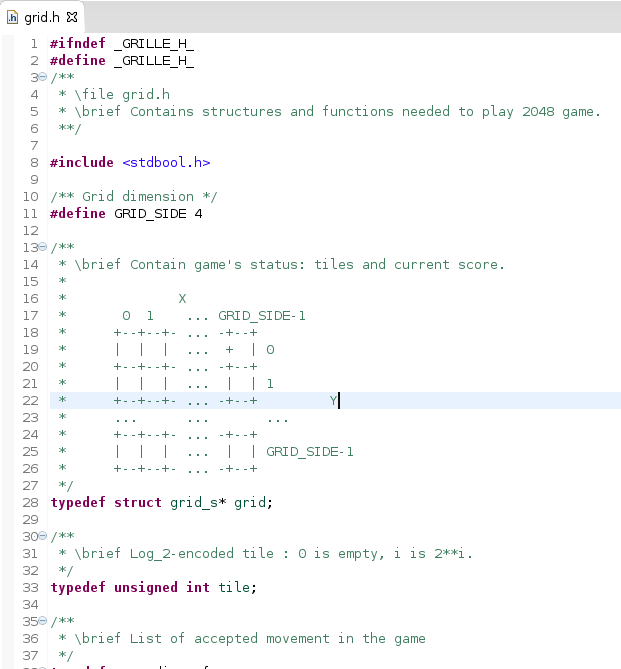
\includegraphics[scale=0.6]{grid_h.png}
\end{figure}

\begin{figure}
   \caption{\label{grille_couleur} Deuxi\`eme version d'affichage de la grille}
   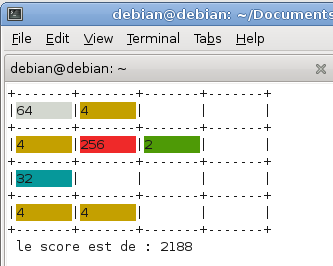
\includegraphics[width=7cm]{grille_couleur.png}
\end{figure}

\begin{figure}
   \caption{\label{test} R\'esultat ex\'ecution des tests}
   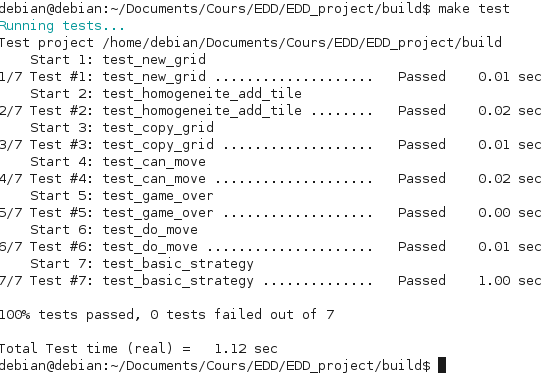
\includegraphics[scale=0.6]{test.png}
\end{figure}
\end{document}